\documentclass[urlcolor=blue,dvipsnames]{beamer}

\usepackage[utf8]{inputenc}
\usepackage{fancybox,fancyvrb}
\usepackage{environ,xspace,empheq}

\usepackage{tikz}
\usetikzlibrary{arrows.meta,decorations.markings,decorations.pathreplacing,fadings,positioning}

\hypersetup{colorlinks,linkcolor=,urlcolor=cyan}

\beamertemplatenavigationsymbolsempty
\setbeamertemplate{footline}[frame number]
\usetheme{Pittsburgh}

\newcommand\enumnum[1]{{\renewcommand{\insertenumlabel}{#1}%
      \usebeamertemplate{enumerate item} \,}}

\newcommand{\grad}{\nabla}
\newcommand{\ih}{\boldsymbol{\hat{\textbf{\i}}}}
\newcommand{\jh}{\boldsymbol{\hat{\textbf{\j}}}}
\newcommand{\vF}{\boldsymbol{\vec{\textbf{F}}}}
\newcommand{\Matlab}{\textsc{Matlab}\xspace}
\newcommand{\Octave}{\textsc{Octave}\xspace}


\title{7.1 Laplace Transforms \\ (starting from the definition)}

\subtitle{a lesson for MATH F302 Differential Equations}

\author{Ed Bueler, Dept.~of Mathematics and Statistics, UAF}

\date{\tiny \today}


\begin{document}
\setbeamertemplate{itemize item}{$\bullet$}
\setbeamertemplate{itemize subitem}{$\circ$}
\renewcommand{\thefootnote}{{\color{green} \arabic{footnote}}}

\begin{frame}
\titlepage

\centerline{\tiny for textbook: \, D. Zill, \emph{A First Course in Differential Equations with Modeling Applications}, 11th ed.}
%\color{green!40!blue}
\end{frame}

\newcommand{\LL}[1]{\mathcal{L}\left\{#1\right\}}

\begin{frame}{the definition}

\begin{itemize}
\item the \alert{Laplace transform} of a function $f(t)$ defined on $(0,\infty)$ is
    $$\alert{\boxed{\LL{f(t)} = \int_0^\infty e^{-st} f(t)\,dt}}$$

\vspace{-2mm}
    \begin{itemize}
    \item this is the book's notation
    \end{itemize}
\item the \alert{result} of applying the Laplace transform \alert{is a function of s}
    \begin{itemize}
    \item  so slightly better notation would be
    $$\LL{f}(s) = \int_0^\infty e^{-st} f(t)\,dt$$
    \item a common (and good) way to write it is
    $$F(s) = \int_0^\infty e^{-st} f(t)\,dt$$
    \end{itemize}
\end{itemize}
\end{frame}


\begin{frame}{why do we use $\mathcal{L}$ in differential equations?}

\begin{itemize}
\item why do we use
    $$\LL{f(t)} = \int_0^\infty e^{-st} f(t)\,dt \quad?$$
\item because the Laplace transform \alert{converts a linear DE} (in $t$) \alert{into an algebra problem} (in $s$)
    \begin{itemize}
    \item this is especially useful for solving \emph{nonhomogeneous} DEs
    \item \dots it's how many engineers think about nonhomogeneous DEs
    \item the Laplace transform \emph{linear}, that is,
\begin{align*}
\LL{f(t) + g(t)} &= \LL{f(t)} + \LL{g(t)}, \, \text{ and} \\
\LL{\alpha f(t)} &= \alpha \LL{f(t)}
\end{align*}
    \item the Laplace transform is basically limited to linear DEs
    \end{itemize}
\end{itemize}
\end{frame}


\begin{frame}{practice with integrals on $[a,\infty)$}

\begin{itemize}
\item a Laplace transform is an integral $\int_0^\infty \dots$
\item we need practice!
\item \emph{practice 1}.  compute
    $$\int_2^\infty e^{-3t}\,dt = \hspace{60mm}$$

\vspace{10mm}
\hfill $=\frac{1}{3} e^{-6}$
\item \emph{practice 2}.  compute and sketch
    $$\int_1^\infty \frac{1}{t}\,dt = \hspace{60mm}$$

\vspace{10mm}
\hfill $=+\infty$
\end{itemize}
\end{frame}


\begin{frame}{practice integrals, cont.}

\begin{itemize}
\item \emph{practice 3}.  compute and sketch
    $$\int_0^\infty t e^{-t}\,dt = \hspace{60mm}$$

\vspace{20mm}
\hfill $=+1$

\vspace{10mm}
\end{itemize}
\end{frame}


\begin{frame}{Laplace transforms, from the definition}

\begin{itemize}
\item the technique in Chapter 7 requires pre-computing the Laplace transforms of some familiar functions, and then using these to solve DEs
\item \emph{example 1}.  compute $\LL{e^{kt}}$

\vspace{25mm}
\item \emph{example 2}.  compute $\LL{1}$

\vspace{25mm}
\end{itemize}
\end{frame}


\begin{frame}{from the definition, cont.}

\begin{itemize}
\item \emph{example 3}.  compute $\LL{t}$

\vspace{30mm}
\item \emph{example 4}.  compute $\LL{\cos(kt)}$

\vspace{35mm}
\end{itemize}
\end{frame}


\begin{frame}{from the definition, cont.$^2$}

\begin{itemize}
\item \emph{example 5}.  compute $\LL{t^n}$

\vspace{50mm}
\hfill $\begin{matrix}
        \LL{t^n} = \frac{n}{s} \LL{t^{n-1}} \\ \\
        \implies \LL{t^n} = \frac{n!}{s^{n+1}}
        \end{matrix}$
\end{itemize}
\end{frame}


\begin{frame}{first table}

\begin{center}
\includegraphics[width=0.75\textwidth]{figs/laplacetable.pdf}
\end{center}

\vspace{-4mm}
\begin{itemize}
\item you will have a table like this on quizzes and exams
\item \emph{and} it is a fair question to ask you to show any one from the definition
\end{itemize}
\end{frame}


\begin{frame}{another example from the definition}

\begin{itemize}
\item \emph{example 6}.  compute $\LL{f}$ if
    $$f(t) = \begin{cases} 0, & 0 \le t < a \\
                           1, & t > a \end{cases} \hspace{50mm}$$

\vspace{35mm}
\hfill $\LL{f} = \frac{e^{-as}}{s}$
\item several WebAssign problems are piecewise like this
\end{itemize}
\end{frame}


\begin{frame}{key fact from \S 7.2}

\begin{itemize}
\item \emph{example 7}.  let $Y(s) = \LL{y(t)}$.  use the definition to show
    $$\LL{y'(t)} = s Y(s) - y(0)$$

\vspace{50mm}
\end{itemize}
\end{frame}


\begin{frame}{an \emph{actual} example}

\begin{itemize}
\item so far, examples just compute $\LL{f(t)}$ for particular $f(t)$
\item \dots they \emph{don't} show how $\mathcal{L}$ is actually used!
\item \emph{example 8}.  solve by using $\mathcal{L}$:
    $$y'+5y=t, \,y(0)=0 \hspace{50mm}$$
\end{itemize}

\vspace{40mm}
\hfill \footnotesize $y(t) = \frac{1}{25} (e^{-5t} - 1) + \frac{t}{5}$
\end{frame}


\begin{frame}{the old way, to check}

\begin{itemize}
\item \emph{example 8'}.  solve by using Chapter 2 methods:
    $$y'+5y=t, \,y(0)=0 \hspace{50mm}$$
\end{itemize}

\vspace{60mm}
\end{frame}


\begin{frame}{can you always compute $\mathcal{L}$?}

\begin{itemize}
\item your function $f(t)$ has to be defined on the interval $[0,\infty)$ so you can do the integral $\int_0^\infty e^{-st} f(t)\,dt$
\item even then, the function has to \emph{not blow-up too fast}
    \begin{itemize}
    \item \emph{bad example.}  try to compute
      $$\LL{e^{t^2}} = \hspace{70mm}$$
    \end{itemize}
\item the result may not be defined for all $s$
    \begin{itemize}
    \item \emph{example.}  explain why this result only makes sense for $s>7$:
      $$\LL{e^{7t}} = \frac{1}{s-7}\hspace{70mm}$$
    \end{itemize}

\end{itemize}
\end{frame}


\begin{frame}{can you always compute $\mathcal{L}$? \, cont.}

\begin{itemize}
\item \emph{definition.}  a function $f(t)$, defined on $[0,\infty)$, is of \emph{exponential order} $c$ if there are constants $M$ and $c$ so that
    $$|f(t)| \le M e^{ct}$$
for all $t$ in $[0,\infty)$
\end{itemize}

\bigskip
\begin{theorem}
if $f(t)$ is piecewise continuous on $[0,\infty)$ and of exponential order $c$ then $\LL{f(t)}$ is defined for $s>c$
\end{theorem}
\end{frame}


\begin{frame}{the Laplace transform strategy}

\begin{center}
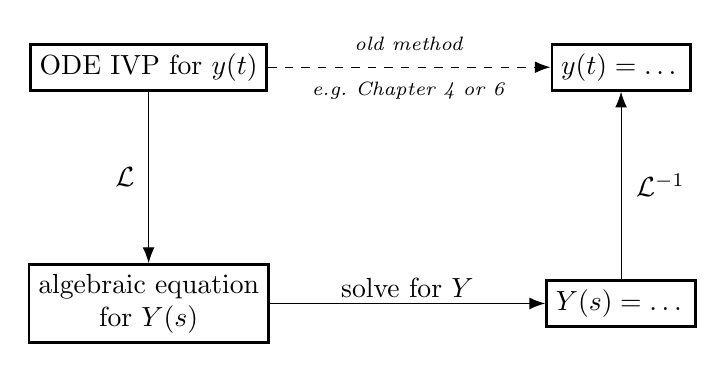
\begin{tikzpicture}[scale=1.0,>={Latex[length=2mm]},
  component/.style={rectangle,draw,fill=white,align=center,line width=1pt}]

\draw (-3,3) node[component] (ode) {ODE IVP for $y(t)$};
\draw (-3,0) node[component] (Leqn) {algebraic equation \\ for $Y(s)$};
\draw (3,0) node[component] (Lsoln)   {$Y(s)=\dots$};
\draw (3,3) node[component] (odesoln)   {$y(t)=\dots$};
\path
   (ode) edge[->] node[xshift=-3mm] {$\mathcal{L}$} (Leqn)
   (Leqn) edge[->] node[yshift=2mm] {solve for $Y$} (Lsoln)
   (Lsoln) edge[->] node[xshift=+5mm] {$\mathcal{L}^{-1}$} (odesoln)
   (ode) edge[dashed,->] node[yshift=3mm] {\scriptsize \emph{old method}} node[yshift=-3mm] {\scriptsize \emph{e.g.~Chapter 4 or 6}} (odesoln);

\end{tikzpicture}
\end{center}

\begin{itemize}
\item example 8 used this strategy
\item we get serious about this strategy in \S 7.2 and \S 7.3
\end{itemize}
\end{frame}


\begin{frame}{beating a dead DE \dots}

\begin{itemize}
\item by then end of this Chapter we will have a \emph{third} good way of solving linear, constant-coefficient DEs:
     \begin{itemize}
     \item[Chapter 4] use auxiliary equation and undetermined coefficients
     \item[Chapter 6] use power series
     \item[Chapter 7] use Laplace transform

\bigskip
     \item both homogenous and nonhomogeneous
     \item all these methods use linearity \dots they are \emph{not} suited to nonlinear DEs
     \item only Chapter 6 methods are well-suited to variable coefficients
     \item in Chapter 8 we will get one more method
     \end{itemize}
\end{itemize}
\end{frame}



\begin{frame}{expectations}

\begin{itemize}
\item just watching this video is \emph{not} enough!
     \begin{itemize}
     \item see ``found online'' videos and stuff at

     \centerline{\href{https://bueler.github.io/math302/week11.html}{\tt \color{cyan} bueler.github.io/math302/week11.html}}
     \item \emph{read} section 7.1 in the textbook
     \item \emph{do} the WebAssign exercises for section 7.1
     \end{itemize}
\end{itemize}
\end{frame}

\end{document}

